\documentclass[11pt]{article}
 
\usepackage[margin=1in]{geometry}
\usepackage{amsmath,amssymb,amsthm}
\usepackage{booktabs,array}
\usepackage{enumitem}
\usepackage{xcolor}
\usepackage{microtype}
\usepackage{float}
\usepackage{tikz}
\usetikzlibrary{arrows.meta,positioning,calc,decorations.pathreplacing}
\usepackage[most]{tcolorbox}
\usepackage[colorlinks=true,linkcolor=blue!50!black,citecolor=blue!50!black,urlcolor=blue!50!black]{hyperref}
 
\setlist{itemsep=2pt,topsep=4pt}
\setlength{\parskip}{3pt}
\renewcommand{\arraystretch}{1.15}
 
% Placeholder for things I could not fill in (shown in red). Delete when done.
\newcommand{\todo}[1]{\textcolor{red!70!black}{\textbf{[FILL:}~#1\textbf{]}}}
 
% Notation
\newcommand{\E}{\mathbb{E}}
\renewcommand{\Pr}{\mathbb{P}}
\newcommand{\nb}{\mathcal{N}}   % neighbourhood in the similarity graph (kept apart from N_i)
 
% Theorem environments: one shared counter, numbered within sections
\theoremstyle{plain}
\newtheorem{theorem}{Theorem}[section]
\newtheorem{lemma}[theorem]{Lemma}
\newtheorem{proposition}[theorem]{Proposition}
\theoremstyle{definition}
\newtheorem{definition}[theorem]{Definition}
\newtheorem{example}[theorem]{Example}
\theoremstyle{remark}
\newtheorem{remark}[theorem]{Remark}
 
\title{Formalizing Resistance in a Social Reward Economy}
\author{Aaron Avram}
\date{October 15, 2026}
 
\begin{document}
\maketitle
 
\begin{abstract}
\noindent
A dominant norm can benefit most of a population while systematically harming a minority.
This report formalizes a \emph{resistant subgroup}: a set of agents together with a set of states
in which every member does badly under the dominant policy.
Finding the strongest such subgroup is a maximum-weight biclique problem, which is NP-hard,
so I give a decentralized formation algorithm instead. Agents estimate their own rewards from experience,
leaders certify candidate groups with a union-bound argument, and a Jaccard nearest-neighbour graph limits who talks to whom.
I prove three things: every committed group is a genuine biclique with a certified platform (soundness),
the algorithm terminates in at most $|G|$ iterations, and under a planted-group assumption it recovers exactly the planted groups
once every agent has observed each relevant state enough times, with an explicit bound on how many.
\end{abstract}
 
 
 
% ============================================================
\section{Introduction}
% ============================================================
 
\subsection{Motivation}
A social norm is a pattern of behaviour that a population settles into because deviating from it is costly.
A norm can be welfare-maximizing for the population as a whole and still leave some agents
persistently worse off than they would be under an alternative. When enough of those agents are
hurt in the \emph{same} situations, they have a shared reason to resist the norm and a shared basis for
organizing around a different one.
 
\textit{Learning Norms}~\cite{learningnorms} gives a formal definition of a single social reward economy and a
model that converges reliably to the welfare-optimal norm. \textit{Social Reward Economies}~\cite{sre}
describes how these ideas extend to settings where several norms compete and several reward economies coexist in
the same system, and defines a resistant subgroup there. \textit{Social Reward Economies} defines a resistant subgroup
as a group which views the dominant norm as detrimental rather than beneficial and
forms an alternative reward economy to better reflect the interests and needs of its members.
The example used in the paper to illustrate such a group was the \#MeToo movement within Hollywood.
Models of the first kind describe convergence to \emph{one} norm. They say little about a minority that
the winning norm leaves behind, or about how such a minority could find itself.
 
\subsection{The problem}
This report addresses three questions, in order:
\begin{enumerate}[label=\textbf{Q\arabic*.},leftmargin=2.5em]
    \item \textbf{Definition.} What is a resistant subgroup, precisely enough to be optimized or tested for?
    \item \textbf{Mechanism.} Agents see only their own rewards, and only noisily. How can a group of agents who
          share grievances identify each other without a central coordinator?
    \item \textbf{Guarantee.} Under what conditions does the mechanism provably produce the intended subgroup, and how much
          experience do agents need before it does?
\end{enumerate}
 
\subsection{Approach and contributions}
The report separates the answers into three layers, summarized in Table~\ref{tab:layers}.
 
\begin{table}[h]
\centering
\begin{tabular}{@{}p{2.6cm}p{4.1cm}p{3.4cm}p{3.9cm}@{}}
\toprule
\textbf{Layer} & \textbf{Object} & \textbf{Role} & \textbf{Guarantee} \\
\midrule
Specification & Admissible pairs $(H,T)$ and strength $\Phi$ (bicliques) & Defines what a resistant subgroup is and what to maximize & None algorithmic; the target and benchmark \\
Realization & Leader proposals, a union-bound certificate, votes & What agents actually run & Soundness; termination; exact recovery of planted groups \\
Communication & Jaccard $\ell$-nearest-neighbour graph & Who considers whom & Reach within two hops under a degree condition \\
\bottomrule
\end{tabular}
\caption{The three layers of the model and what each one guarantees.}
\label{tab:layers}
\end{table}
 
\noindent The main results are:
\begin{itemize}
    \item \textbf{Definition} (Section~\ref{sec:def}). A resistant subgroup is a biclique in the agent--state graph of negative expected rewards.
          The strongest one maximizes total expected loss. I connect this to the maximum edge-weight biclique problem and give a relaxation
          with exact coordinate updates.
    \item \textbf{Algorithm} (Section~\ref{sec:mech}). Agents keep running averages of their own rewards and treat a state as a grievance only when
          the estimate is confidently negative. A leader admits agents while the union bound certifies that the group still shares most of the leader's
          grievances. Competing proposals are resolved by a vote.
    \item \textbf{Analysis} (Section~\ref{sec:analysis}). Soundness holds with no structural assumption (Proposition~\ref{prop:sound}).
          Termination holds within $|G|$ iterations (Proposition~\ref{prop:term}).
          Under a planted-group assumption, exactly the planted groups commit in the first formation epoch with probability at least $1-\delta$,
          once agents have enough observations (Theorem~\ref{thm:formation}).
\end{itemize}
 
\subsection{Background and related work}
Finding a maximum edge biclique in a bipartite graph is NP-complete~\cite{peeters}, and the maximal bicliques of a relation are exactly the formal
concepts studied in formal concept analysis~\cite{fca}. The formation algorithm is a coalition-formation procedure,
and the confidence-based rule for deciding who belongs to a group is in the spirit of clustering of bandits~\cite{club}, where a
similarity graph over users is pruned as confidence intervals separate them.
The estimation guarantees use Hoeffding's inequality~\cite{hoeffding}.
Related questions about how a committed minority can overturn an established convention are studied empirically in~\cite{centola};
I return to this in Section~\ref{sec:discussion}.
 
\subsection{Organization}
Section~\ref{sec:setup} sets up the model and gives a small worked example.
Section~\ref{sec:def} defines resistant subgroups.
Section~\ref{sec:mech} describes how agents estimate, certify and form groups.
Section~\ref{sec:analysis} states and proves the guarantees.
Section~\ref{sec:discussion} discusses what is and is not covered and what comes next.
 
% ============================================================
\section{Set up}\label{sec:setup}
% ============================================================
\subsection{Model}
The basic setup for the system is as follows:
\begin{itemize}
    \item There is a set of agents $G$.
    \item A set of states $S$, where $s \in S$ has probability $p(s)$ of occurring.
    \item For each $s \in S$ there is a set $A(s)$ of possible actions in state $s$.
    \item A policy is a function that maps each $s \in S$ to a probability distribution over $A(s)$.
          Fix a \emph{dominant policy} $\pi_d$.
    \item Each agent $i \in G$ has a fixed reward $u_i(s, a)$ for action $a \in A(s)$ in state $s \in S$.
    \item Each agent $i$ has an expected reward under a policy $\pi$ in state $s$:
    \[ U_i(s, \pi) = \E_{a \sim \pi(s)}\Big[u_i(s, a)\Big]. \]
    \item For each $i \in G$ there is a set of states $N_i \subseteq S$, the \emph{disagreement set} of $i$, defined as
    \[ N_i = \{ s \in S : U_i(s, \pi_d) < -\tau \} \]
    for a fixed constant $\tau > 0$.
\end{itemize}
The system runs in discrete time. At each step $t \in \mathbb N$ it enters a state $s(t)$ sampled independently from $p$.
For simplicity I assume the dominant policy stays fixed throughout, and that at each step every agent acts and observes its own reward.
 
\subsection{Notation}
Table~\ref{tab:notation} collects the notation used throughout.
\begin{table}[!ht]
\centering
\small
\begin{tabular}{@{}lp{12.2cm}@{}}
\toprule
\textbf{Symbol} & \textbf{Meaning} \\
\midrule
$G,\ S,\ p(s)$ & agents, states, state probabilities; $|G|$ is the number of agents \\
$\pi_d,\ U_i(s,\pi_d)$ & dominant policy; agent $i$'s expected reward in state $s$ under it \\
$w_i(s)$ & grievance $\max(0,-U_i(s,\pi_d))$ \\
$N_i$ & disagreement set $\{s : U_i(s,\pi_d)<-\tau\}$, with margin $\tau$ \\
$(H,T),\ \Phi,\ \Phi_\lambda$ & subgroup (agents $H$, platform $T$); strength and its relaxation \\
$\hat v_i(s),\ n_i(s)$ & running mean of $i$'s observed rewards at $s$, and the visit count \\
$\hat N_i,\ \hat w_i$ & estimated disagreement set (confident states only) and estimated grievance \\
$\eta,\ n_0,\ B,\ \delta$ & estimation error constant, count threshold, reward bound, failure probability \\
$L_k(i),\ \hat L_k(i)$ & mass of leader $k$'s grievances that $i$ does not share (true and estimated) \\
$\epsilon$ & tolerance in the union-bound admission rule \\
$\ell,\ \nb(k)$ & number of neighbours in the similarity graph; neighbourhood of $k$ \\
$K,\ \Delta,\ p_{\min}$ & number of formation epochs, spacing between them, minimum significant state probability \\
$H_r,\ T_r$ & planted groups and their platforms (Section~\ref{sec:analysis}) \\
$m,\ t,\ q,\ \gamma,\ \mu$ & group size, platform mass, private mass, depth margin, separation fraction \\
\bottomrule
\end{tabular}
\caption{Notation.}
\label{tab:notation}
\end{table}
 
\subsection{A worked example}
\begin{example}\label{ex:toy}
Take five agents $a_1,\dots,a_5$ and four equally likely states $s_1,\dots,s_4$ ($p(s)=1/4$), with $\tau = 0.5$.
The table gives $U_i(s,\pi_d)$; negative entries below $-\tau$ are the grievances.
\begin{center}
\small
\begin{tabular}{@{}c cccc c@{}}
\toprule
 & $s_1$ & $s_2$ & $s_3$ & $s_4$ & $N_i$ \\
\midrule
$a_1$ & $-2.0$ & $-1.5$ & $\phantom{-}1.0$ & $\phantom{-}0.5$ & $\{s_1,s_2\}$ \\
$a_2$ & $-1.8$ & $-2.0$ & $-1.0$ & $\phantom{-}1.0$ & $\{s_1,s_2,s_3\}$ \\
$a_3$ & $-1.5$ & $-1.2$ & $\phantom{-}0.5$ & $\phantom{-}1.0$ & $\{s_1,s_2\}$ \\
$a_4$ & $\phantom{-}1.0$ & $-2.0$ & $-1.5$ & $-1.0$ & $\{s_2,s_3,s_4\}$ \\
$a_5$ & $\phantom{-}1.0$ & $\phantom{-}0.5$ & $\phantom{-}1.0$ & $\phantom{-}1.0$ & $\varnothing$ \\
\bottomrule
\end{tabular}
\end{center}
The strongest admissible pair is $(\{a_1,a_2,a_3\},\{s_1,s_2\})$ with $\Phi = \tfrac14(2+1.5+1.8+2+1.5+1.2)=2.5$.
For comparison, $(\{a_1,\dots,a_4\},\{s_2\})$ has $\Phi=1.675$ and $(\{a_2,a_4\},\{s_2,s_3\})$ has $\Phi=1.625$.
Figure~\ref{fig:toy} shows the agent--state graph. The same example is reused in Section~\ref{sec:mech} to illustrate the formation algorithm.
\end{example}
 
\begin{figure}[!ht]
\centering
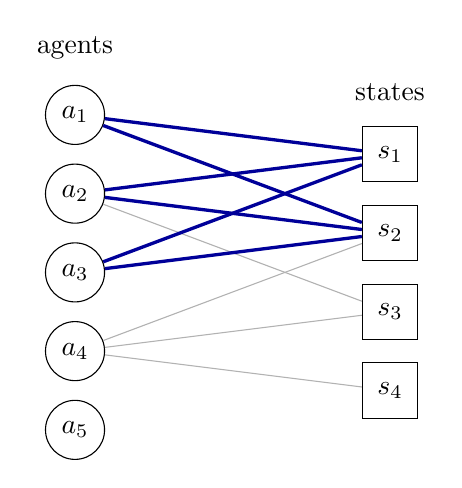
\begin{tikzpicture}[
  agent/.style={circle,draw,minimum size=7.5mm,inner sep=0pt},
  state/.style={rectangle,draw,minimum size=7mm,inner sep=0pt},
  e/.style={gray!60},
  hl/.style={very thick,blue!60!black}]
  \foreach \i/\y in {1/4,2/3,3/2,4/1,5/0}{\node[agent] (a\i) at (0,\y) {$a_\i$};}
  \foreach \j/\y in {1/3.5,2/2.5,3/1.5,4/0.5}{\node[state] (s\j) at (4,\y) {$s_\j$};}
  % background edges (all grievances)
  \foreach \i/\j in {2/3,4/2,4/3,4/4}{\draw[e] (a\i) -- (s\j);}
  % the strongest biclique
  \foreach \i in {1,2,3}{\foreach \j in {1,2}{\draw[hl] (a\i) -- (s\j);}}
  \node[above=2mm of a1] {agents};
  \node[above=2mm of s1] {states};
\end{tikzpicture}
\caption{Agent--state graph of Example~\ref{ex:toy}. An edge joins $i$ and $s$ when $s\in N_i$.
The thick edges form the strongest biclique $(\{a_1,a_2,a_3\},\{s_1,s_2\})$. Agent $a_5$ has no grievances.}
\label{fig:toy}
\end{figure}
 
% ============================================================
\section{Defining Resistance Theoretically}\label{sec:def}
% ============================================================
\begin{definition}
    The \emph{grievance} of an agent $i$ in a state $s$ is
    \[ w_i(s) = \max(0, -U_i(s,\pi_d)). \]
    It measures how dissatisfied $i$ is with the dominant norm in state $s$.
\end{definition}
\begin{remark}
    $N_i$ is the set of states in which $i$'s grievance exceeds $\tau$, that is, the disagreement set of $i$.
\end{remark}
\begin{definition}
    A \emph{subgroup} is a pair $(H, T)$ of a set of agents $H \subseteq G$ and a set of states $T \subseteq S$ (its \emph{platform}).
    The pair is \emph{admissible} if $T \subseteq \bigcap_{i \in H}N_i$.
\end{definition}
\begin{definition}
    The \emph{strength} of a subgroup is
    \[ \Phi(H, T) = \sum_{i \in H}\sum_{s \in T}p(s)w_i(s). \]
    A \emph{maximally resistant subgroup} is an admissible pair that maximizes $\Phi$.
\end{definition}
 
\paragraph{Why this definition.} Membership is about \emph{shared} grievances: members need to be badly off in the same states, but not
by the same amount. An earlier version of this report measured the total disagreement of a group together with a ``friction'' term for how different
members' grievance profiles are. Total disagreement alone grows with the group, so the friction constraint needed a tolerance parameter.
With the biclique definition the trade-off is built in: adding an agent can only shrink the states all members share, and adding a state can only shrink the set of agents negative on it.
 
\subsection{Connection to bicliques}
Build a bipartite graph with agents on one side and states on the other, and weight $W[i, s] = p(s)w_i(s)$ on the edge between $i$ and $s$ when $s \in N_i$.
An admissible pair is a biclique: a bipartite subgraph in which every agent of $H$ is joined to every state in $T$.
The strength $\Phi$ is the sum of its edge weights. Finding a maximum edge biclique is NP-complete even without weights~\cite{peeters}.
 
\begin{remark}[Closure]
Because all weights are nonnegative, for a fixed $H$ the best platform is everything the members share, $T(H)=\bigcap_{i\in H}N_i$,
and for a fixed $T$ the best group is everyone negative on all of $T$, $H(T)=\{i: T\subseteq N_i\}$. The problem therefore reduces to choosing $H$,
and the fixed points of these two maps are the maximal bicliques (formal concepts~\cite{fca}).
Enumerating them gives an exact baseline on small instances, which is useful for evaluating the algorithms below.
\end{remark}
 
\subsection{A relaxation}
The hardness comes from the all-or-nothing requirement $T \subseteq N_i$. I relax it by charging each $i \in H$ for the states in $T$
where $i$ actually benefits from $\pi_d$. Let
\[ V[i, s] = p(s)\max(0, U_i(s, \pi_d)), \qquad M_\lambda = W - \lambda V, \qquad
\Phi_\lambda(H, T) = \sum_{i \in H}\sum_{s \in T}M_\lambda[i, s]. \]
The parameter $\lambda\ge 0$ sets how strict the group is. As $\lambda \to \infty$ any state in $T$ where a member benefits becomes arbitrarily costly, which recovers
the exact biclique problem (up to the margin $\tau$). On admissible pairs $V = 0$, so $\Phi_\lambda = \Phi$.
 
For a relaxation the optimal pair has a closed form in each coordinate. For a fixed $T$ the best $H$ is $\{ i: r_i > 0 \}$ where
$r_i = \sum_{s \in T}M_\lambda[i, s]$, and for a fixed $H$ the best $T$ is $\{ s : c_s > 0 \}$ where $c_s = \sum_{i \in H}M_\lambda[i, s]$.
Alternating these two steps increases $\Phi_\lambda$ monotonically. In the rest of the report $\Phi_\lambda$ is used only to \emph{rank} competing proposals.
 
% ============================================================
\section{Subgroup Formation Mechanics}\label{sec:mech}
% ============================================================
Agents do not know their rewards in advance. This section describes how they estimate them, what they treat as a grievance,
how a leader certifies a group, who talks to whom, and when all of this runs.
 
\subsection{Estimating rewards}
Each agent $i$ keeps a running mean $\hat v_i(s)$ of the rewards it has observed in state $s$ under $\pi_d$, initialized at $0$, and the visit count $n_i(s)$.
When $s(t)=s$ and $i$ observes the reward $u_i(s,a)$ for $a\sim\pi_d(s)$,
\[ \hat v_i(s) \;\leftarrow\; \frac{1}{n_i(s)+1}\Big(u_i(s, a) + n_i(s)\hat v_i(s)\Big), \qquad n_i(s)\leftarrow n_i(s)+1, \]
and otherwise both are unchanged. Agents compute all of the quantities of Section~\ref{sec:def} from $\hat v_i(s)$ in place of $U_i(s,\pi_d)$,
and a hat marks such an estimate: $\hat w_i(s)=\max(0,-\hat v_i(s))$, and so on.
Estimates are shared between agents, and I assume messages are exact and honest.
 
\subsection{Confident disagreement sets}
A state counts as a grievance only when the estimate is confidently negative. For a fixed error constant $\eta > 0$ and count threshold $n_0$ define
\[ \hat{N}_i = \{ s \in S : n_i(s) \geq n_0,\ \hat{v}_i(s) < -\tau - \eta \}. \]
The count threshold and the extra margin $\eta$ guarantee that $\hat N_i\subseteq N_i$ with high probability (Proposition~\ref{prop:sound}), so a state is never
counted as a grievance because of sampling noise.
 
\subsection{The union-bound certificate}
Fix a leader $k$ and a group $H\ni k$. A state in $N_k$ is lost to the group exactly when some member does not share it, so
\[ \bigcap_{i\in H}N_i \;=\; N_k \setminus \bigcup_{i \in H}(N_k\setminus N_i). \]
Writing $L_k(i)=\sum_{s\in N_k\setminus N_i}p(s)$ for the mass of $k$'s grievances that $i$ does not share, the union bound gives
\begin{equation}\label{eq:ub}
p\Big(\bigcap_{i \in H}N_i\Big)\;\ge\; p(N_k)-\sum_{i\in H}L_k(i).
\end{equation}
So a leader can certify that the group keeps most of its own platform by adding up \emph{pairwise} quantities, each computed between the leader and one candidate.
This avoids the trap of purely pairwise rules: all pairwise overlaps can be large while the common intersection is empty.
Agents cannot compute $L_k$, since it uses the true sets, so they use
\[ \hat{L}_k(i)=\sum_{s \in \hat{N}_k \setminus \hat{N}_i}p(s). \]
Proposition~\ref{prop:sound} shows that the same inequality holds for $\hat L_k$ and $\hat N$ with high probability.
The bound is tight when the sets $N_k\setminus N_i$ are disjoint across members; it can be loose by a factor of up to $|H|-1$ when members all lack the same private states of $k$ (Section~\ref{sec:discussion}).
 
\subsection{Who talks to whom}
To decide which agents interact during formation I define a similarity on the set of agents, the weighted Jaccard similarity of their estimated grievances:
\[ \operatorname{sim}(i, j) = \frac{\sum_{s \in S}p(s)\min\{ \hat{w}_i(s), \hat{w}_j(s) \}}{\sum_{s \in S}p(s)\max \{ \hat{w}_i(s), \hat{w}_j(s) \}}. \]
Only states where both agents have a grievance contribute to the numerator, and a grievance held by one agent but not the other counts against them in the denominator.
The $\ell$-nearest-neighbour graph on $G$ connects each agent to the $\ell$ agents most similar to it; $\nb(k)$ is the neighbourhood of $k$. This graph only decides which agents a leader considers.
Membership is decided by the certificate, so a bridge agent can be a neighbour of two groups without merging them.
 
\subsection{The formation algorithm}
\emph{Leaders} are agents with $\hat N_k\neq\varnothing$. A leader is always a member of its own group. Ties between proposals are broken by agent id.
 
\begin{tcolorbox}[colback=gray!5,colframe=gray!60,title={\textbf{Algorithm: one formation epoch}},fonttitle=\small,left=4pt,right=4pt]
\begin{enumerate}[label=(\arabic*),leftmargin=2.2em,itemsep=3pt]
    \item \textbf{Neighbours.} Each leader $k$ collects $\nb(k)$, its $\ell$ nearest neighbours in the Jaccard graph.
    \item \textbf{Pool.} Every member of $\nb(k)$ forwards its own $\ell$ nearest neighbours to $k$, so $k$'s pool of candidates is $\nb(k)\cup\nb(\nb(k))$.
    \item \textbf{Propose.} $k$ sorts the pool by $\hat L_k(i)$ and admits candidates in this order, stopping at the first one for which
    \[ \hat{L}_k(i) + \sum_{j \in H_k}\hat{L}_k(j) \leq \epsilon\cdot p(\hat N_k) \]
    fails, for a tolerance $\epsilon\in(0,1)$. The admitted set is $H_k$ (which contains $k$). The proposal is the pair $(H_k,\hat T_k)$ with
    $\hat T_k=\bigcap_{i\in H_k}\hat N_i$, with score $\sigma_k=\Phi_\lambda(H_k,\hat T_k)$.
    \item \textbf{Vote.} Each agent identifies with the highest-scoring proposal that includes it.
    \item \textbf{Commit.} A leader $k$ commits to $H_k$ if every member of $H_k$ identifies with its proposal.
    \item \textbf{Remove.} Committed agents are no longer considered in this epoch.
    \item \textbf{Repeat or stop.} Repeat (1)--(6) on the remaining agents until no leaders remain.
\end{enumerate}
\end{tcolorbox}
 
Because the budget is cumulative, the admitted set always satisfies
\begin{equation}\label{eq:budget}
\sum_{i \in H_k}\hat{L}_k(i) \leq \epsilon\, p(\hat{N}_k).
\end{equation}
 
\begin{example}[Example~\ref{ex:toy} continued]
Take $\epsilon = 0.2$ and exact estimates. Leader $a_1$ has $p(N_1)=1/2$, so its budget is $0.1$. The costs are $L_1(a_2)=L_1(a_3)=0$ and $L_1(a_4)=p(\{s_1\})=0.25$.
It admits $a_2$ and $a_3$ and rejects $a_4$, proposing $(\{a_1,a_2,a_3\},\{s_1,s_2\})$ with score $2.5$. Leader $a_3$ proposes the same group with the same score.
Leader $a_2$, whose grievance set also contains the private state $s_3$, has budget $0.15$ but pays $L_2(a_1)=L_2(a_3)=0.25$, so it admits nobody and proposes $(\{a_2\},N_2)$ with score $1.2$.
Leader $a_4$ similarly proposes only itself. All members of the top proposal vote for it, and the tie between $a_1$ and $a_3$ is broken by id, so $a_1$ commits.
This shows that a leader with many private grievances makes a poor leader: the certificate charges it for each of them.
\end{example}
 
\subsection{The epoch schedule}
Formation does not run at every time step but on a timeline of formation epochs (Figure~\ref{fig:timeline}), controlled by two parameters: $K$, the maximum number of formation epochs, and $\Delta$, the spacing between them.
To prevent premature formation, the first epoch starts only once every agent is \emph{ready}: $n_i(s)\ge n_0$ for all $i$ and all $s$ with $p(s)\ge p_{\min}$,
where $p_{\min}$ is a minimum probability for a state to be considered significant. Readiness depends only on counts, so each agent can check it locally.
Epochs then run at times $t^{(1)}<t^{(2)}<\dots$ with $t^{(j+1)}=t^{(j)}+\Delta$. At each epoch the Jaccard graph is recomputed from the current estimates on the agents that are still uncommitted.
The process stops when no leaders remain or after $K$ epochs. Committed agents stay committed.
 
\begin{figure}[h]
\centering
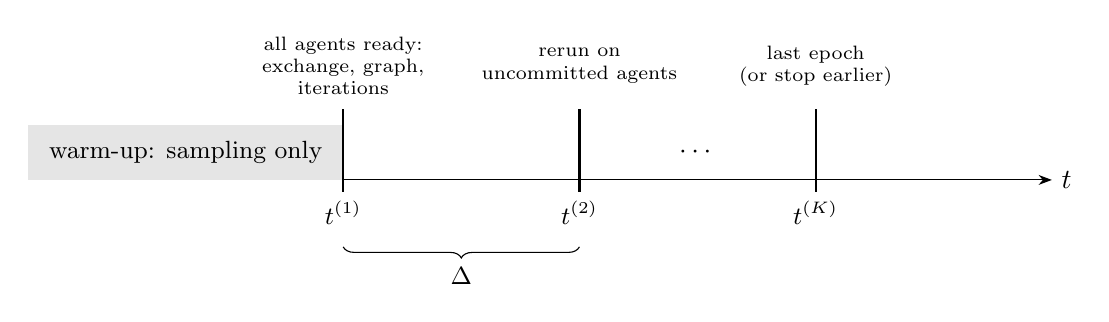
\begin{tikzpicture}[x=1cm,y=1cm,>={Stealth}]
  \draw[->] (0,0) -- (13,0) node[right] {$t$};
  \fill[gray!20] (0,0) rectangle (4,0.7);
  \node at (2,0.35) {\small warm-up: sampling only};
  \foreach \x/\lab in {4/1,7/2,10/K}{
     \draw[thick] (\x,-0.15) -- (\x,0.9);
     \ifnum\x=10 \node[below] at (\x,-0.15) {\small $t^{(K)}$}; \else \node[below] at (\x,-0.15) {\small $t^{(\lab)}$}; \fi
  }
  \node[align=center,font=\scriptsize] at (4.0,1.45) {all agents ready:\\exchange, graph,\\iterations};
  \node[align=center,font=\scriptsize] at (7.0,1.45) {rerun on\\uncommitted agents};
  \node[align=center,font=\scriptsize] at (10.0,1.45) {last epoch\\(or stop earlier)};
  \draw[decorate,decoration={brace,amplitude=4pt,mirror}] (4,-0.85) -- (7,-0.85) node[midway,below=4pt] {\small $\Delta$};
  \node at (8.5,0.35) {$\cdots$};
\end{tikzpicture}
\caption{Timeline of the model: a warm-up in which agents only sample, then up to $K$ formation epochs spaced $\Delta$ apart.}
\label{fig:timeline}
\end{figure}
 
% ============================================================
\section{Theoretical Analysis}\label{sec:analysis}
% ============================================================
This section gives guarantees for the model above. The first part (soundness and termination) holds for every instance; the second part (exact recovery) needs structural assumptions on the instance.
Most of the section is technical, and it serves to justify the definitions of Section~\ref{sec:mech} rigorously.
 
\subsection{Standing assumptions}
(i) $\pi_d$ is fixed. (ii) $p(s)$ is known to all agents. (iii) Messages are exact and honest. (iv) Rewards satisfy $|u_i(s,a)|\le B$ for some $B>0$.
(v) At each step the state is drawn independently of the past, every agent acts and draws $a\sim\pi_d(s)$ independently, and observes $u_i(s,a)$;
hence $\hat v_i(s)$ is the mean of $n_i(s)$ i.i.d.\ draws with mean $U_i(s,\pi_d)$.
Assumption (v) simplifies the calculations. Removing the requirement that every agent acts at every step changes the analysis only in Lemma~\ref{lem:counts}, which then needs a larger bound on the time to reach the count $n_0$.
 
\subsection{Estimation}
\begin{lemma}[Estimation]\label{lem:est}
Let $\theta=\eta^2/(2B^2)$ and
\[ n_0=\Big\lceil \theta^{-1}\log\frac{2|G||S|}{\delta(1-e^{-\theta})}\Big\rceil. \]
Then the event
\[ E:\quad |\hat{v}_i(s) - U_i(s, \pi_d)| \leq \eta\ \text{ for all } i,s \text{ with } n_i(s) \geq n_0,\ \text{at all times} \]
holds with probability at least $1-\delta$.
\end{lemma}
\begin{proof}
Fix $(i,s)$ and let $\bar u_{i,n}$ be the mean of the first $n$ rewards that $i$ observes in state $s$. Rewards lie in $[-B,B]$, so Hoeffding's inequality gives
\[ \Pr\big(|\bar u_{i,n}-U_i(s,\pi_d)|\ge\eta\big)\le 2e^{-n\theta}. \]
A union bound over $n\ge n_0$ gives
\[ \Pr\big(\exists\, n\ge n_0:\ |\bar u_{i,n}-U_i(s,\pi_d)|\ge\eta\big)\;\le\;\sum_{n= n_0}^\infty 2e^{-n\theta}\;=\;\frac{2e^{-n_0\theta}}{1-e^{-\theta}}\;\le\;\frac{\delta}{|G||S|}, \]
where the last step is the choice of $n_0$. At any time at which $n_i(s)\ge n_0$, $\hat v_i(s)=\bar u_{i,n_i(s)}$, so this covers every time at once. A union bound over the $|G||S|$ pairs $(i,s)$ shows $\Pr(E^c)\le\delta$.
\end{proof}
 
\begin{lemma}[Visit counts]\label{lem:counts}
Let $T\subseteq S$ and $p_{\min}(T)=\min_{s\in T}p(s)$. If
\[ t\;\ge\;\frac{\max\{2n_0,\ 8\log(|G||S|/\delta)\}}{p_{\min}(T)}, \]
then with probability at least $1-\delta$, $n_i(s)\ge n_0$ for every agent $i$ and every $s\in T$ at time $t$.
\end{lemma}
\begin{proof}
$n_i(s)$ is binomial with mean $tp(s)$, so the multiplicative Chernoff bound gives $\Pr(n_i(s)\le tp(s)/2)\le e^{-tp(s)/8}$. For $s\in T$,
$tp(s)/2\ge n_0$ and $tp(s)/8\ge\log(|G||S|/\delta)$, so
\[ \Pr\Big(\bigcup_{i\in G,\,s\in T}\{n_i(s)< n_0\}\Big)\le\sum_{i\in G,\,s\in T}e^{-tp(s)/8}\le\sum_{i,s}\frac{\delta}{|G||S|}\le\delta. \qedhere \]
\end{proof}
 
\subsection{Soundness}
\begin{proposition}[Soundness]\label{prop:sound}
On $E$ the following hold.
\begin{enumerate}[label=(\alph*)]
    \item $\hat N_i \subseteq N_i$ for every $i$.
    \item For any leader $k$ and any set $H \ni k$,
    \[ p\Big(\bigcap_{i \in H}N_i\Big) \;\ge\; p\Big(\bigcap_{i \in H}\hat{N}_i\Big) \;\ge\; p(\hat{N}_k) - \sum_{i \in H}\hat{L}_k(i). \]
    \item If $H=H_k$ satisfies~\eqref{eq:budget}, then $(H_k, \hat{T}_k)$ is admissible, $p(\hat{T}_k) \ge (1 - \epsilon)\,p(\hat{N}_k)$, and
    \[ \Phi_\lambda(H_k, \hat{T}_k) \;\ge\; \tau\,|H_k|\,(1 - \epsilon)\,p(\hat{N}_k). \]
\end{enumerate}
\end{proposition}
\begin{proof}
(a) If $s\in\hat N_i$ then $n_i(s)\ge n_0$, so on $E$, $U_i(s,\pi_d)\le\hat v_i(s)+\eta<-\tau$, i.e.\ $s\in N_i$.
 
(b) The second inequality is the union bound: since $k\in H$,
$\bigcap_{i \in H}\hat{N}_i=\hat{N}_k\setminus\bigcup_{i \in H}(\hat{N}_k\setminus\hat{N}_i)$, hence
\[ p\Big(\bigcap_{i\in H}\hat N_i\Big)\ \ge\ p(\hat N_k)-\sum_{i\in H}p(\hat N_k\setminus\hat N_i). \]
The first inequality follows from (a), since $\hat N_i\subseteq N_i$ implies $\bigcap_{i\in H}\hat N_i\subseteq\bigcap_{i\in H}N_i$.
 
(c) Admissibility follows from (a) and the mass bound from (b) together with~\eqref{eq:budget}. For the last bound, $V[i,s]=0$ for $s\in\hat T_k$ because $U_i(s,\pi_d)<-\tau<0$,
so $\Phi_\lambda=\Phi$ on admissible pairs; and $w_i(s)>\tau$ on $N_i$, so $\Phi(H,T)\ge\tau|H|p(T)$ for every admissible $(H,T)$.
\end{proof}
 
Proposition~\ref{prop:sound} uses no structural assumption on the instance. Every committed group is a genuine biclique, with a platform whose mass is certified by the leader.
 
\subsection{Termination}
\begin{proposition}[Termination]\label{prop:term}
Each iteration of the formation algorithm commits at least one group, so a formation epoch stops after at most $|G|$ iterations.
\end{proposition}
\begin{remark}
The proof does not use any of the assumptions above.
\end{remark}
\begin{proof}
Order the proposals of an iteration by $(\sigma_k,\text{id})$ and let $k^*$ be the top one. Each member of $H_{k^*}$ identifies with the highest-ranked proposal that includes it, and $H_{k^*}$ is a proposal that includes it and is ranked highest overall.
So every member of $H_{k^*}$ identifies with $k^*$, and $k^*$ commits. Each iteration therefore removes at least one agent (the leader), and the epoch ends after at most $|G|$ iterations.
\end{proof}
 
\subsection{Formation of planted groups}
To say what the algorithm should find, consider disjoint groups $H_1,\dots,H_R\subseteq G$ with platforms $T_1,\dots,T_R\subseteq S$.
For each $r$ write $m=|H_r|\ge2$, $t=p(T_r)$, and let $q$ be the private-mass bound below. (These all depend on $r$; the index is dropped when no confusion arises.) Assume $\epsilon\in(0,1)$.
 
\begin{enumerate}[label=\textbf{(P\arabic*)},leftmargin=3.2em,itemsep=4pt]
    \setcounter{enumi}{-1}
    \item \textbf{Significance.} $p(s)\ge p_{\min}$ for every $s\in\bigcup_rT_r$.
    \item \textbf{Depth.} For all $i\in H_r$ and $s\in T_r$, $U_i(s,\pi_d)\le-\tau-\gamma$, with $\gamma>2\eta$.
    \item \textbf{Private mass.} $p(N_i\setminus T_r)\le q$ for all $i\in H_r$, with $(m-1)q\le\epsilon t$.
    \item \textbf{Separation.} Every agent $o\notin H_r$ satisfies $p(T_r\setminus N_o)\ge\mu t$, with $\mu>\epsilon(1+q/t)$.
    \item \textbf{No background grievances.} Agents outside $\bigcup_rH_r$ have $N_o=\varnothing$.
    \item[\textbf{(G)}] \textbf{Graph reach.} At the first formation epoch, the undirected version of the $\ell$-nearest-neighbour graph, restricted to $H_r$,
          has minimum degree at least $\lceil(m-1)/2\rceil$, for each $r$.
\end{enumerate}
 
In words: members are clearly negative on the platform (P1), have little grievance mass outside it (P2), every outsider misses a substantial part of it (P3), and the leader can reach all its group through the graph (G).
Section~\ref{sec:discussion} discusses how restrictive each of these is.
 
\begin{lemma}[Graph reach]\label{lem:graph}
Under (G), any two members of $H_r$ are adjacent or share a common neighbour in $H_r$. In particular, for every $k\in H_r$,
\[ H_r\subseteq\{k\}\cup\nb(k)\cup\nb(\nb(k)). \]
\end{lemma}
\begin{proof}
Suppose $u,v\in H_r$ are not adjacent. Each has at least $\lceil(m-1)/2\rceil$ neighbours in $H_r$, and these lie in $H_r\setminus\{u,v\}$, a set of size $m-2$. Since
$2\lceil(m-1)/2\rceil\ge m-1>m-2$, the two neighbour sets intersect.
\end{proof}
 
\begin{remark}[When (G) holds]
Suppose $\ell\ge\lceil(m-1)/2\rceil$ and every estimated member--member similarity exceeds every estimated member--outsider similarity. Then the $\ell$ nearest neighbours of a member
include $\min\{\ell,m-1\}\ge\lceil(m-1)/2\rceil$ members, so (G) holds. Groups with $m>2\ell+1$ can fragment even under these conditions.
\end{remark}
 
\begin{theorem}[Formation]\label{thm:formation}
Assume the standing assumptions, (P0)--(P4) and (G), and let the first formation epoch be the first time at which every agent is ready.
Then with probability at least $1-\delta$, in the first formation epoch exactly the groups $H_1,\dots,H_R$ commit, each with a platform $\hat T_r\supseteq T_r$ that is admissible and satisfies
$p(\hat T_r)\ge(1-\epsilon)\,p(\hat N_k)$ for the leader $k$ that commits. No other agent commits, and the algorithm then stops.
Moreover, with probability at least $1-2\delta$ this first epoch occurs no later than
\[ t_0=\frac{\max\{2n_0,\ 8\log(|G||S|/\delta)\}}{p_{\min}}. \]
\end{theorem}
 
\begin{proof}
Work on the event $E$ of Lemma~\ref{lem:est}, which has probability at least $1-\delta$. By (P0) and the definition of readiness, $n_i(s)\ge n_0$ for all $i$ and all $s\in\bigcup_rT_r$ at the first epoch.
Fix $r$ and a leader $k\in H_r$.
\begin{enumerate}[label=\textbf{Step \arabic*.},leftmargin=4.6em,itemsep=4pt]
    \item \emph{The platform is certified.} For $i\in H_r$ and $s\in T_r$, on $E$,
    $\hat v_i(s)\le U_i(s,\pi_d)+\eta\le-\tau-\gamma+\eta<-\tau-\eta$, as $\gamma>2\eta$. So $T_r\subseteq\hat N_i$ for every $i\in H_r$, and hence
    $t\le p(\hat N_k)\le p(N_k)\le t+q$.
    \item \emph{The pool contains the group.} By Lemma~\ref{lem:graph}, $H_r$ lies in the two-hop pool of $k$.
    \item \emph{Members are cheap.} For $i\in H_r$, $\hat N_k\setminus\hat N_i\subseteq\hat N_k\setminus T_r\subseteq N_k\setminus T_r$ (using Step 1 and Proposition~\ref{prop:sound}(a)), so $\hat L_k(i)\le q$. Thus
    \[ \sum_{i\in H_r}\hat L_k(i)\le(m-1)q\le\epsilon t\le\epsilon\,p(\hat N_k). \]
    \item \emph{Outsiders are expensive.} Let $o\notin H_r$ be any other agent. Since $T_r\subseteq\hat N_k$ and $\hat N_o\subseteq N_o$, we have $T_r\setminus N_o\subseteq\hat N_k\setminus\hat N_o$, so by (P3)
    \[ \hat L_k(o)\ \ge\ \mu t\ >\ \epsilon(t+q)\ \ge\ \epsilon\,p(\hat N_k). \]
    (If $N_o=\varnothing$ then $\hat L_k(o)=p(\hat N_k)\ge t>\epsilon\,p(\hat N_k)$.) Moreover $q\le\epsilon t/(m-1)\le\epsilon t<\mu t$, so every member is sorted before every outsider.
    \item \emph{The proposal.} By Steps 3 and 4 the sorted list begins with all of $H_r\setminus\{k\}$, which are all admitted within the budget, and the first outsider violates the budget on its own. Hence $H_k=H_r$.
    \item \emph{The vote.} By Step 5 every leader in $H_r$ proposes $H_r$. By (P4) the only leaders are members of planted groups, and a leader in $H_{r'}$ proposes $H_{r'}$, which is disjoint from $H_r$.
    So the proposals that include a member of $H_r$ are exactly the $m$ proposals $H_r$, with scores $\sigma_{k'}$, $k'\in H_r$. All members rank these identically, so they identify with the same leader $k^*$, and $k^*$ commits.
    \item \emph{Conclusion.} Proposition~\ref{prop:sound}(c) gives the stated properties of the committed groups, and $T_r\subseteq\hat T_r$ by Step 1. Every committed agent is removed, and the remaining agents have $N_o=\varnothing$, so there are no leaders and the algorithm stops.
\end{enumerate}
For the second claim, apply Lemma~\ref{lem:counts} with $T=S_{\ge p_{\min}}=\{s:p(s)\ge p_{\min}\}$: with probability at least $1-\delta$ every agent has $n_i(s)\ge n_0$ for all $s\in T$ by time $t_0$,
so all agents are ready by $t_0$. A union bound with $E$ gives probability at least $1-2\delta$.
\end{proof}
 
\begin{remark}[Sample complexity]
Only the platform states need to be certified, so the time to formation scales as $1/(\gamma^2p_{\min})$ with $|S|$ appearing only in the logarithm.
Taking $\eta$ just below $\gamma/2$ gives $n_0\approx(8B^2/\gamma^2)\log\big(2|G||S|/(\delta(1-e^{-\theta}))\big)$.
\end{remark}
 
% ============================================================
\section{Discussion and Next Steps}\label{sec:discussion}
% ============================================================
 
\subsection{What has been shown}
The report defines a resistant subgroup as a biclique of shared grievances and gives a decentralized procedure for finding such groups from noisy individual experience.
Two properties hold on every instance: a committed group is always a genuine biclique with a certified platform (soundness), and the procedure always terminates (at most $|G|$ iterations).
Exact recovery of the intended groups needs structural assumptions, and under them the time to formation scales as $1/(\gamma^2 p_{\min})$.
The three layers play different roles: the biclique definition states what is wanted, the certificate and votes realize it, and the similarity graph only limits communication. Only the middle layer carries guarantees on its own.
 
\subsection{How restrictive are the assumptions?}
\paragraph{Private mass (P2) costs a factor of $m$.}
The union bound charges a private state of the leader once per member, so (P2) requires $q\le\epsilon t/(m-1)$.
For $m=20$ and $\epsilon=0.2$ this allows private grievances of only about $1\%$ of the platform mass, so members' grievances must be almost nested.
If the leader instead admits agents while $p\big(\bigcap_{i\in C}\hat N_i\big)\ge(1-\epsilon)\,p(\hat N_k)$, i.e.\ it charges the \emph{union} of missing states and not the \emph{sum},
the same proof goes through with (P2) replaced by $q\le\epsilon t/(1-\epsilon)$ (and $\mu>q/t$), with no dependence on $m$. Both rules are sound. The union bound is the right tool only if the leader cannot hold its members' sets;
with all estimates shared, the exact intersection is strictly better.
 
\paragraph{Background grievances (P4).}
Agents outside the planted groups are assumed to have no grievances. A simple relaxation replaces ``leader'' by $p(\hat N_k)\ge\tau_c$ and allows background agents with grievance mass below $\tau_c$, small enough that they fail the budget when a group leader considers them.
The hard case is a background agent whose grievances lie inside a platform: its proposal absorbs the group and competes by score, and the outcome is determined by the ranking by $\Phi_\lambda$. Then the planted group need not be $\Phi$-optimal and the right claim is a maximality statement that I have not proved.
 
\paragraph{Graph reach (G).}
(G) is assumed, not derived. The remark after Lemma~\ref{lem:graph} gives a sufficient condition in terms of similarities, but the Jaccard similarity penalizes a member's private grievances, which the biclique definition and the certificate do not. A member with large private grievances can be a certified fit for a leader yet not be among its nearest neighbours.
A containment-based similarity, ranking candidates by $\hat L_k(i)$ directly, would match the certificate exactly but is asymmetric, so the degree argument would need to be redone for a directed graph.
 
\paragraph{Permanent commits and warm-up.}
Committed agents are never reconsidered. This is harmless for correctness, since a committed group stays a valid biclique when $\pi_d$ and the rewards are fixed. It is why formation must wait for the warm-up:
a premature commit could be valid but partial, and it could not be repaired. Alternatives are to re-run formation from scratch at each epoch, which makes the output at every epoch after warm-up correct and stable, or to add an explicit leave rule that lets a member go only when it
\emph{certifiably} mismatches the group (using the optimistic cost $p(\hat N_k\cap\{s:\hat v_i(s)>-\tau+\eta\})$) while joining uses the pessimistic cost $\hat L_k(i)$, which gives hysteresis from the confidence margins. The leave rule needs a margin assumption on outsiders in order to evict early false members.
 
\paragraph{Other modelling assumptions.}
(i) The dominant policy is fixed, whereas a resistant group that grows could change it (Section~\ref{sec:next}). (ii) Messages are honest and exact; noise or deception would add error terms to $\hat L$. (iii) Every agent acts at every step; asynchronous visits only change Lemma~\ref{lem:counts}.
(iv) The error constant $\eta$ is common to all agents and states; per-state confidence widths, for example empirical Bernstein bounds, would give faster and less conservative formation.
(v) Groups are disjoint. Overlapping bicliques, where an agent belongs to two groups with different platforms, are a natural case that the vote resolves only by score.
 
\subsection{Next steps}\label{sec:next}
\begin{enumerate}[label=\textbf{\arabic*.},leftmargin=2em,itemsep=4pt]
    \item \textbf{Simulation.} Test the theory empirically on planted instances and measure how much slack the conditions have. The proposed design is in Table~\ref{tab:sim}.
    \item \textbf{Relax the assumptions.} Prove the exact-intersection variant, the small-mass background case, and a certified leave rule. Study when the maximum-$\Phi$ biclique and the planted group coincide, and whether the greedy procedure has an approximation guarantee for $\Phi$.
    \item \textbf{After formation.} Once a group has formed, it needs a norm of its own. Run the dynamics of \textit{Learning Norms} (reputation, status, and gossip) inside the group, and show convergence to a norm that benefits all its members. A sufficient condition is that an alternative policy $\pi_H$ exists with $U_i(s,\pi_H)\ge 0$ on the platform for every member $i$; this is an assumption and not yet something agents can check.
    \item \textbf{Feedback on the dominant norm.} If the resistant group grows large enough, the dominant policy changes and the sets $N_i$ with it. This closes the loop between formation and norm dynamics and connects to the tipping-point results for committed minorities~\cite{centola}.
    \item \textbf{Realistic communication.} Replace honest exact messages with noisy or strategic ones. Gaussian noise on messages can be analysed as an extra error term; deception raises the question of whether a group can be formed by agents that can misreport their grievances.
    \item \textbf{Alternative realizations of the same specification.} Platform dynamics (alternating maximization of $\Phi_\lambda$, which needs only each agent's own utilities) and a marginal-contribution coalition game (an exact potential game) realize the same biclique objective with local-optimum guarantees instead of the certificate.
\end{enumerate}
 
\begin{table}[h]
\centering
\small
\begin{tabular}{@{}p{3.7cm}p{6.0cm}p{5.2cm}@{}}
\toprule
\textbf{Factor} & \textbf{Values} & \textbf{Measured} \\
\midrule
Group size $m$ and private mass $q$ & sweep $q/t$ across the threshold $\epsilon/(m-1)$ & recovery with the union bound vs.\ the exact-intersection rule \\
Depth $\gamma$ and $\eta$ & $\gamma/2$ against $\eta$ & time to formation vs.\ the bound $\max\{2n_0,\cdot\}/p_{\min}$ \\
Neighbours $\ell$ and group size & $\ell$ below, at and above $(m-1)/2$ & whether (G) holds, and recovery \\
Background grievance mass & none, small, large idiosyncratic & false commits, absorbed groups \\
Epochs $K$, spacing $\Delta$ & $K=1$ vs.\ larger $K$; warm-up on/off & partial commits, time to stop \\
\bottomrule
\end{tabular}
\caption{Proposed simulation design. Baselines: exact biclique enumeration on small instances, spectral clustering on the similarity matrix, and a centralized greedy.
Metrics throughout: Jaccard overlap between recovered and planted groups, false-commit rate, number of messages.}
\label{tab:sim}
\end{table}
 
% ============================================================
\begin{thebibliography}{9}
\bibitem{learningnorms} {Learning Norms: V.~Sharma and P.~Marbach, Learning Common Norms in Multi-Agent Systems, 2026}
\bibitem{sre} {Social Reward Economies: P.~Marbach and S.~Jiang, Social Reward Economies: The Dynamic Architecture of Cohesion, Polarization, Resistance and Manipulation, 2026}
\bibitem{peeters} R.~Peeters. The maximum edge biclique problem is NP-complete. \textit{Discrete Applied Mathematics}, 131(3):651--654, 2003.
\bibitem{fca} B.~Ganter and R.~Wille. \textit{Formal Concept Analysis: Mathematical Foundations}. Springer, 1999.
\bibitem{hoeffding} W.~Hoeffding. Probability inequalities for sums of bounded random variables. \textit{Journal of the American Statistical Association}, 58(301):13--30, 1963.
\bibitem{club} C.~Gentile, S.~Li and G.~Zappella. Online clustering of bandits. In \textit{Proceedings of the 31st International Conference on Machine Learning}, 2014.
\bibitem{centola} D.~Centola, J.~Becker, D.~Brackbill and A.~Baronchelli. Experimental evidence for tipping points in social convention. \textit{Science}, 360(6393):1116--1119, 2018.
\end{thebibliography}
 
\end{document}